% Options for packages loaded elsewhere
\PassOptionsToPackage{unicode}{hyperref}
\PassOptionsToPackage{hyphens}{url}
\PassOptionsToPackage{dvipsnames,svgnames,x11names}{xcolor}
%
\documentclass[
  letterpaper,
  DIV=11,
  numbers=noendperiod]{scrartcl}

\usepackage{amsmath,amssymb}
\usepackage{iftex}
\ifPDFTeX
  \usepackage[T1]{fontenc}
  \usepackage[utf8]{inputenc}
  \usepackage{textcomp} % provide euro and other symbols
\else % if luatex or xetex
  \usepackage{unicode-math}
  \defaultfontfeatures{Scale=MatchLowercase}
  \defaultfontfeatures[\rmfamily]{Ligatures=TeX,Scale=1}
\fi
\usepackage{lmodern}
\ifPDFTeX\else  
    % xetex/luatex font selection
\fi
% Use upquote if available, for straight quotes in verbatim environments
\IfFileExists{upquote.sty}{\usepackage{upquote}}{}
\IfFileExists{microtype.sty}{% use microtype if available
  \usepackage[]{microtype}
  \UseMicrotypeSet[protrusion]{basicmath} % disable protrusion for tt fonts
}{}
\makeatletter
\@ifundefined{KOMAClassName}{% if non-KOMA class
  \IfFileExists{parskip.sty}{%
    \usepackage{parskip}
  }{% else
    \setlength{\parindent}{0pt}
    \setlength{\parskip}{6pt plus 2pt minus 1pt}}
}{% if KOMA class
  \KOMAoptions{parskip=half}}
\makeatother
\usepackage{xcolor}
\setlength{\emergencystretch}{3em} % prevent overfull lines
\setcounter{secnumdepth}{5}
% Make \paragraph and \subparagraph free-standing
\makeatletter
\ifx\paragraph\undefined\else
  \let\oldparagraph\paragraph
  \renewcommand{\paragraph}{
    \@ifstar
      \xxxParagraphStar
      \xxxParagraphNoStar
  }
  \newcommand{\xxxParagraphStar}[1]{\oldparagraph*{#1}\mbox{}}
  \newcommand{\xxxParagraphNoStar}[1]{\oldparagraph{#1}\mbox{}}
\fi
\ifx\subparagraph\undefined\else
  \let\oldsubparagraph\subparagraph
  \renewcommand{\subparagraph}{
    \@ifstar
      \xxxSubParagraphStar
      \xxxSubParagraphNoStar
  }
  \newcommand{\xxxSubParagraphStar}[1]{\oldsubparagraph*{#1}\mbox{}}
  \newcommand{\xxxSubParagraphNoStar}[1]{\oldsubparagraph{#1}\mbox{}}
\fi
\makeatother


\providecommand{\tightlist}{%
  \setlength{\itemsep}{0pt}\setlength{\parskip}{0pt}}\usepackage{longtable,booktabs,array}
\usepackage{calc} % for calculating minipage widths
% Correct order of tables after \paragraph or \subparagraph
\usepackage{etoolbox}
\makeatletter
\patchcmd\longtable{\par}{\if@noskipsec\mbox{}\fi\par}{}{}
\makeatother
% Allow footnotes in longtable head/foot
\IfFileExists{footnotehyper.sty}{\usepackage{footnotehyper}}{\usepackage{footnote}}
\makesavenoteenv{longtable}
\usepackage{graphicx}
\makeatletter
\def\maxwidth{\ifdim\Gin@nat@width>\linewidth\linewidth\else\Gin@nat@width\fi}
\def\maxheight{\ifdim\Gin@nat@height>\textheight\textheight\else\Gin@nat@height\fi}
\makeatother
% Scale images if necessary, so that they will not overflow the page
% margins by default, and it is still possible to overwrite the defaults
% using explicit options in \includegraphics[width, height, ...]{}
\setkeys{Gin}{width=\maxwidth,height=\maxheight,keepaspectratio}
% Set default figure placement to htbp
\makeatletter
\def\fps@figure{htbp}
\makeatother
% definitions for citeproc citations
\NewDocumentCommand\citeproctext{}{}
\NewDocumentCommand\citeproc{mm}{%
  \begingroup\def\citeproctext{#2}\cite{#1}\endgroup}
\makeatletter
 % allow citations to break across lines
 \let\@cite@ofmt\@firstofone
 % avoid brackets around text for \cite:
 \def\@biblabel#1{}
 \def\@cite#1#2{{#1\if@tempswa , #2\fi}}
\makeatother
\newlength{\cslhangindent}
\setlength{\cslhangindent}{1.5em}
\newlength{\csllabelwidth}
\setlength{\csllabelwidth}{3em}
\newenvironment{CSLReferences}[2] % #1 hanging-indent, #2 entry-spacing
 {\begin{list}{}{%
  \setlength{\itemindent}{0pt}
  \setlength{\leftmargin}{0pt}
  \setlength{\parsep}{0pt}
  % turn on hanging indent if param 1 is 1
  \ifodd #1
   \setlength{\leftmargin}{\cslhangindent}
   \setlength{\itemindent}{-1\cslhangindent}
  \fi
  % set entry spacing
  \setlength{\itemsep}{#2\baselineskip}}}
 {\end{list}}
\usepackage{calc}
\newcommand{\CSLBlock}[1]{\hfill\break\parbox[t]{\linewidth}{\strut\ignorespaces#1\strut}}
\newcommand{\CSLLeftMargin}[1]{\parbox[t]{\csllabelwidth}{\strut#1\strut}}
\newcommand{\CSLRightInline}[1]{\parbox[t]{\linewidth - \csllabelwidth}{\strut#1\strut}}
\newcommand{\CSLIndent}[1]{\hspace{\cslhangindent}#1}

\KOMAoption{captions}{tableheading}
\makeatletter
\@ifpackageloaded{caption}{}{\usepackage{caption}}
\AtBeginDocument{%
\ifdefined\contentsname
  \renewcommand*\contentsname{Table of contents}
\else
  \newcommand\contentsname{Table of contents}
\fi
\ifdefined\listfigurename
  \renewcommand*\listfigurename{List of Figures}
\else
  \newcommand\listfigurename{List of Figures}
\fi
\ifdefined\listtablename
  \renewcommand*\listtablename{List of Tables}
\else
  \newcommand\listtablename{List of Tables}
\fi
\ifdefined\figurename
  \renewcommand*\figurename{Figure}
\else
  \newcommand\figurename{Figure}
\fi
\ifdefined\tablename
  \renewcommand*\tablename{Table}
\else
  \newcommand\tablename{Table}
\fi
}
\@ifpackageloaded{float}{}{\usepackage{float}}
\floatstyle{ruled}
\@ifundefined{c@chapter}{\newfloat{codelisting}{h}{lop}}{\newfloat{codelisting}{h}{lop}[chapter]}
\floatname{codelisting}{Listing}
\newcommand*\listoflistings{\listof{codelisting}{List of Listings}}
\makeatother
\makeatletter
\makeatother
\makeatletter
\@ifpackageloaded{caption}{}{\usepackage{caption}}
\@ifpackageloaded{subcaption}{}{\usepackage{subcaption}}
\makeatother

\ifLuaTeX
  \usepackage{selnolig}  % disable illegal ligatures
\fi
\usepackage{bookmark}

\IfFileExists{xurl.sty}{\usepackage{xurl}}{} % add URL line breaks if available
\urlstyle{same} % disable monospaced font for URLs
\hypersetup{
  pdftitle={Electricity Usage in Toronto's Public Facilities: Analyzing the Impact of Building Size on Energy Consumption},
  pdfauthor={Irene Liu},
  colorlinks=true,
  linkcolor={blue},
  filecolor={Maroon},
  citecolor={Blue},
  urlcolor={Blue},
  pdfcreator={LaTeX via pandoc}}


\title{Electricity Usage in Toronto's Public Facilities: Analyzing the
Impact of Building Size on Energy Consumption\thanks{Code and data are
available at:
https://github.com/zilin1017/Toronto\_annual\_energy\_consumption.git.}}
\author{Irene Liu}
\date{September 27, 2024}

\begin{document}
\maketitle
\begin{abstract}
This study examines the relationship between building size(m²) and
electricity consumption(kWh) in Toronto's public facilities. Data from
over 500 buildings, including schools,libraries, and hospitals, show a
consistent positive correlation between GFA and eletricity usage. Larger
facilities, particularly healthcare centers, demonstrate higher energy
consumption per square meter. These results help inform efforts to
improve energy management in Toronto's public buildings.
\end{abstract}

\renewcommand*\contentsname{Table of contents}
{
\hypersetup{linkcolor=}
\setcounter{tocdepth}{3}
\tableofcontents
}

\section{Introduction}\label{introduction}

Public infrastructure, including schools, libraries, healthcare centers,
and government offices, forms the backbone of urban services in any
modern city. As Toronto continues to expand, managing electricity usage
in public buildings becomes increasingly critical. Energy efficiency in
public facilities not only reduces operational costs but also
contributes to environmental goals, such as carbon reduction and climate
change mitigation(Droege 2018).

One of the primary determinants of electricity consumption is building
size, commonly measured as Gross Floor Area (GFA). Larger buildings tend
to consume more energy for lighting, heating, cooling, and equipment
operations, but this relationship is influenced by other factors such as
building type, operational hours, and energy management systems (Hong et
al. 2016). As such, it is crucial for policymakers to understand how
building size and other factors influence electricity consumption in
Toronto's public facilities (Li and Colombier 2009).

Several studies have shown that energy efficiency measures in public
buildings can lead to significant reductions in electricity consumption.
For example, retrofitting large government buildings or healthcare
facilities with modern energy management systems can reduce energy use,
while smaller buildings like libraries and schools often exhibit lower
per-square-meter energy consumption (Scott et al. 2008).

This paper explores the relationship between Property GFA (m²) and
electricity usage (kWh) in over 500 public facilities in Toronto. The
study aims to identify patterns in electricity consumption and provide
insights for optimizing energy use in Toronto's public sector.

\section{Data}\label{sec-data}

\subsection{Raw data}\label{raw-data}

The data used in this paper came from the OpenData Toronto portal
through the library (Gelfand 2022). Data were cleaned and analyzed using
the open source statistical programming language R (R Core Team 2023).
The particular data set used to analyze the Consumption of Energy is the
Annual Energy Consumption Data in 2021 (Toronto Open Data Portal, n.d.).
The following packages helped with the data analysis: tidyverse (Wickham
et al. 2019), here (Müller 2020)), dplyr (Wickham et al. 2023) and
ggplot2 (Wickham 2016) was use for making graphics. All data analysis
was conducted using R (R Core Team 2023).

The data used in this analysis comes from the City of Toronto's Open
Data Portal(Gelfand 2022), specifically focusing on energy consumption
across various property types in Toronto for the year 2021(Toronto Open
Data Portal, n.d.). The dataset consists of 1,802 unique entries, each
representing a specific property in various regions of Toronto. For each
property, the data captures critical metrics such as the building size,
self-reported in gross floor area (GFA) in square meters (m²), and the
total electricity consumption, measured in kilowatt-hours (kWh),
purchased from the grid. No personal or property-specific information is
included. The data was last updated on July 4, 2023, and helps
understand energy usage trends across different building types in
Toronto.

\subsection{Cleaned Data}\label{cleaned-data}

The cleaning process focused on removing irrelevant or incomplete data
to ensure the dataset was suitable for analyzing electricity consumption
patterns in Toronto's public sector. Missing values(NA) were removed
during the data cleaning process, particularly those related to
electricity usage. And buildings that did not meet the size criteria
(less than 30 square meters or greater than 2,500 square meters) were
also filtered out.Additionally, variables irrelevant to the study's
focus were also omitted. Furthermore, the cleaned data retains only the
key variables required for the analysis: property type, electricity use,
floor area, and log-transformed area. This ensures that the final
dataset is both accurate and relevant for understanding electricity
consumption trends across different public facilities in Toronto.

A sample of the cleaned data can be seen in Table~\ref{tbl-1}. The
cleaned analysis dataset is loaded using the R programming language (R
Core Team 2023). The folder structure for this analysis is also
inherited from Professor Rohan Alexander (Alexander 2023). Figures and
tables are then generated using the knitr (Xie 2023) and tidyverse
(Wickham et al. 2019) packages.

\begin{longtable}[]{@{}
  >{\raggedright\arraybackslash}p{(\columnwidth - 6\tabcolsep) * \real{0.3500}}
  >{\centering\arraybackslash}p{(\columnwidth - 6\tabcolsep) * \real{0.2875}}
  >{\centering\arraybackslash}p{(\columnwidth - 6\tabcolsep) * \real{0.1375}}
  >{\centering\arraybackslash}p{(\columnwidth - 6\tabcolsep) * \real{0.2250}}@{}}

\caption{\label{tbl-1}Sample of cleaned data}

\tabularnewline

\toprule\noalign{}
\begin{minipage}[b]{\linewidth}\raggedright
Property Type
\end{minipage} & \begin{minipage}[b]{\linewidth}\centering
Electricity Use (kWh)
\end{minipage} & \begin{minipage}[b]{\linewidth}\centering
Area (m²)
\end{minipage} & \begin{minipage}[b]{\linewidth}\centering
Log of Area (m²)
\end{minipage} \\
\midrule\noalign{}
\endhead
\bottomrule\noalign{}
\endlastfoot
Police Station & 610692.1 & 2395.0 & 7.781138 \\
Other - Public Services & 9469.3 & 40.0 & 3.688880 \\
Other - Lodging/Residential & 76707.2 & 1783.7 & 7.486445 \\
Office & 124585.4 & 934.0 & 6.839476 \\
Heated Swimming Pool & 344470.3 & 1922.0 & 7.561122 \\
Pre-school/Daycare & 81602.7 & 652.0 & 6.480045 \\

\end{longtable}

\subsection{Data Analysis}\label{data-analysis}

\begin{figure}

\centering{

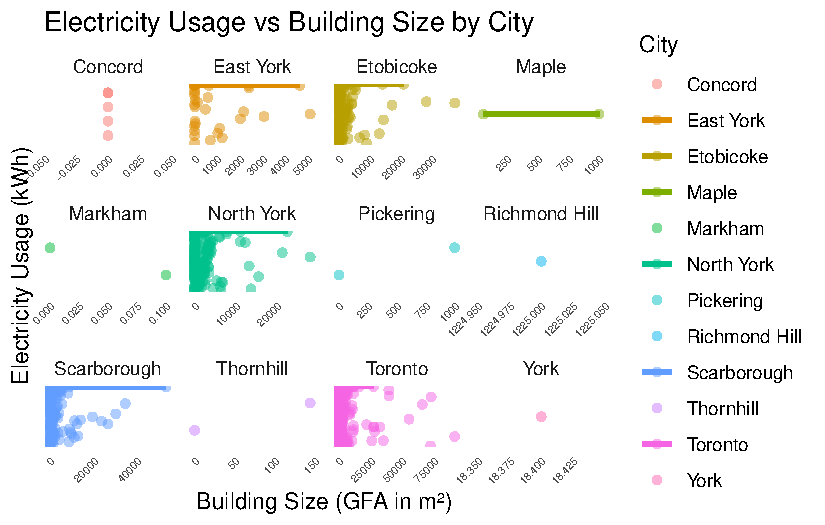
\includegraphics{paper_files/figure-pdf/fig-Area-1.pdf}

}

\caption{\label{fig-Area}Density Plot for Property Area in Toronto}

\end{figure}%

\begin{figure}

\centering{

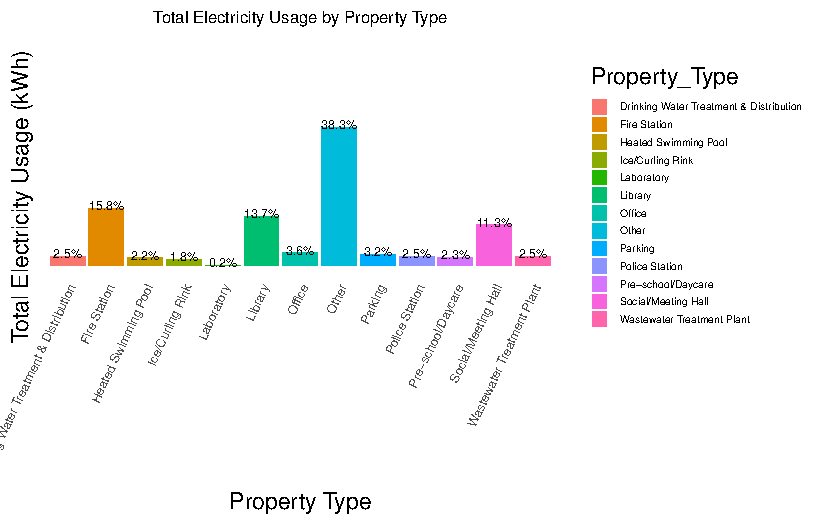
\includegraphics{paper_files/figure-pdf/fig-Property-1.pdf}

}

\caption{\label{fig-Property}Percentage Electricity Usage by Properties}

\end{figure}%

Talk more about it.

And also planes (\textbf{?@fig-planes}). (You can change the height and
width, but don't worry about doing that until you have finished every
other aspect of the paper - Quarto will try to make it look nice and the
defaults usually work well once you have enough text.)

Talk way more about it.

\begin{figure}[H]

{\centering 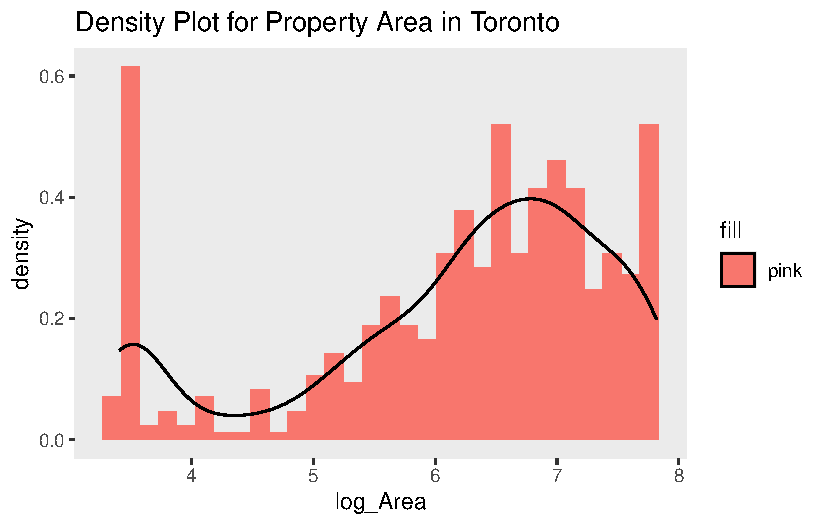
\includegraphics{paper_files/figure-pdf/none-1.pdf}

}

\caption{Relationship between wing length and width}

\end{figure}%

\begin{figure}[H]

{\centering 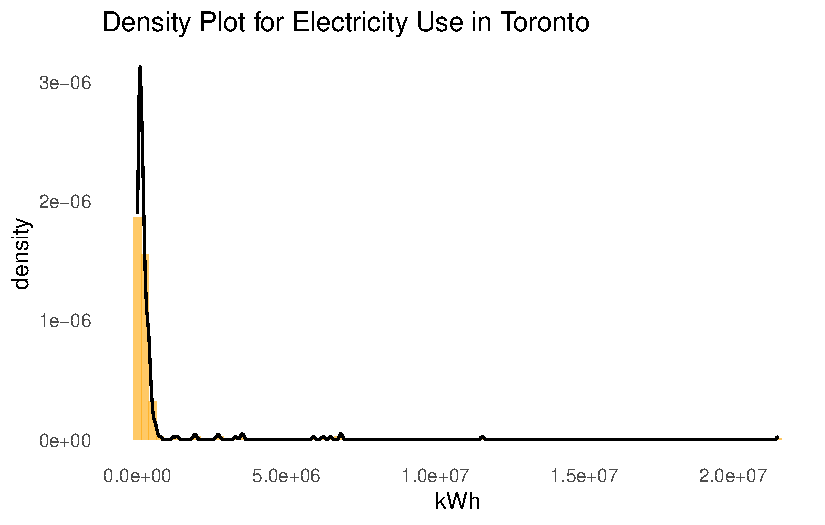
\includegraphics{paper_files/figure-pdf/second-1.pdf}

}

\caption{Relationship between \ldots{}}

\end{figure}%

\section{Results}\label{results}

Our results are summarized in Table~\ref{tbl-modelresults}.

\begin{table}

\caption{\label{tbl-modelresults}}

\centering{

\begin{figure}
\centering
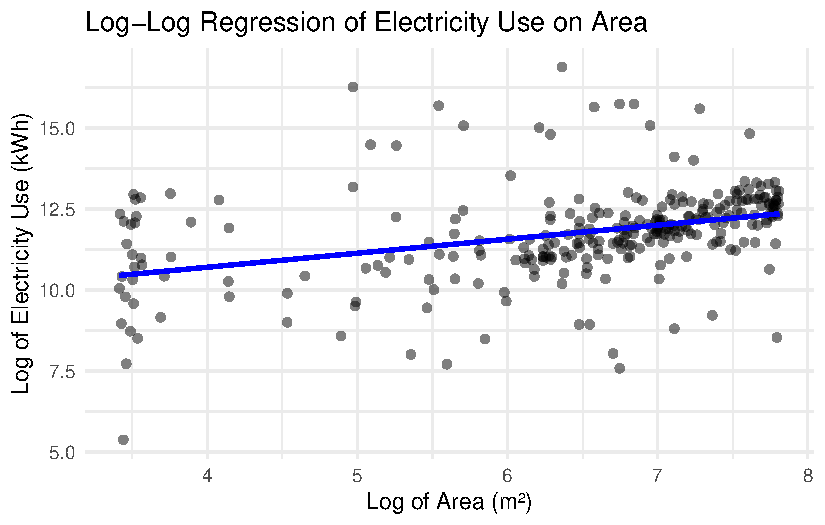
\includegraphics{paper_files/figure-pdf/tbl-modelresults-1.pdf}
\caption{Regression of Electricity Use on Area}
\end{figure}

}

\end{table}%

\section{Discussion}\label{discussion}

\subsection{First discussion point}\label{sec-first-point}

If my paper were 10 pages, then should be be at least 2.5 pages. The
discussion is a chance to show off what you know and what you learnt
from all this.

\subsection{Second discussion point}\label{second-discussion-point}

\subsection{Third discussion point}\label{third-discussion-point}

\subsection{Weaknesses and next steps}\label{weaknesses-and-next-steps}

Weaknesses and next steps should also be included.

\newpage

\appendix

\section*{Appendix}\label{appendix}
\addcontentsline{toc}{section}{Appendix}

\section{Additional data details}\label{additional-data-details}

\section{Model details}\label{sec-model-details}

\subsection{Posterior predictive
check}\label{posterior-predictive-check}

In \textbf{?@fig-ppcheckandposteriorvsprior-1} we implement a posterior
predictive check. This shows\ldots{}

In \textbf{?@fig-ppcheckandposteriorvsprior-2} we compare the posterior
with the prior. This shows\ldots{}

\begin{figure}

\begin{minipage}{0.50\linewidth}
Examining how the model fits, and is affected by, the
data\end{minipage}%

\end{figure}%

\subsection{Diagnostics}\label{diagnostics}

\textbf{?@fig-stanareyouokay-1} is a trace plot. It shows\ldots{} This
suggests\ldots{}

\textbf{?@fig-stanareyouokay-2} is a Rhat plot. It shows\ldots{} This
suggests\ldots{}

\begin{figure}

\begin{minipage}{0.50\linewidth}
Checking the convergence of the MCMC algorithm\end{minipage}%

\end{figure}%

\newpage

\section*{References}\label{references}
\addcontentsline{toc}{section}{References}

\phantomsection\label{refs}
\begin{CSLReferences}{1}{0}
\bibitem[\citeproctext]{ref-rohan}
Alexander, Rohan. 2023. {``Starter Folder.''}
\url{https://github.com/RohanAlexander/starter_folder.git}.

\bibitem[\citeproctext]{ref-droege2018urban}
Droege, Peter. 2018. \emph{Urban Energy Transition: Renewable Strategies
for Cities and Regions}. Elsevier.
\url{https://books-scholarsportal-info.myaccess.library.utoronto.ca/en/read?id=/ebooks/ebooks0/elsevier/2009-12-02/1/9780080453415}.

\bibitem[\citeproctext]{ref-opendt}
Gelfand, Sharla. 2022. \emph{Opendatatoronto: Access the City of Toronto
Open Data Portal}.
\url{https://CRAN.R-project.org/package=opendatatoronto}.

\bibitem[\citeproctext]{ref-hong2016occupant}
Hong, Tianzhen, Sarah C. Taylor-Lange, Simona D'Oca, Da Yan, and Stefano
P. Corgnati. 2016. {``Advances in Research and Applications of
Energy-Related Occupant Behavior in Buildings.''} \emph{Energy and
Buildings} 116: 694--702.
\url{https://doi.org/10.1016/j.enbuild.2015.11.052}.

\bibitem[\citeproctext]{ref-li2009managing}
Li, Jun, and Michel Colombier. 2009. {``Managing Energy Consumption in
China's Large Public Buildings: Policy Challenges and Opportunities.''}
\emph{Energy Policy} 90 (8): 2436--47.
\url{https://doi.org/10.1016/j.jenvman.2008.12.015}.

\bibitem[\citeproctext]{ref-here}
Müller, Kirill. 2020. \emph{Here: A Simpler Way to Find Your Files}.
\url{https://CRAN.R-project.org/package=here}.

\bibitem[\citeproctext]{ref-citeR}
R Core Team. 2023. \emph{R: A Language and Environment for Statistical
Computing}. Vienna, Austria: R Foundation for Statistical Computing.
\url{https://www.R-project.org/}.

\bibitem[\citeproctext]{ref-scott2008impact}
Scott, Michael J., Joseph M. Roop, Robert W. Schultz, David M. Anderson,
and Katherine A. Cort. 2008. {``The Impact of DOE Building Technology
Energy Efficiency Programs on u.s. Employment, Income, and
Investment.''} \emph{Energy Economics} 30 (5): 2283--2301.
\url{https://doi.org/10.1016/j.eneco.2007.09.001}.

\bibitem[\citeproctext]{ref-2021datatoronto}
Toronto Open Data Portal, City of. n.d. {``About Annual Energy
Consumption.''}
\url{https://open.toronto.ca/dataset/annual-energy-consumption/}.

\bibitem[\citeproctext]{ref-ggplot}
Wickham, Hadley. 2016. \emph{Ggplot2: Elegant Graphics for Data
Analysis}. Springer-Verlag New York.
\url{https://ggplot2.tidyverse.org}.

\bibitem[\citeproctext]{ref-tidyverse}
Wickham, Hadley, Mara Averick, Jennifer Bryan, Winston Chang, Lucy
D'Agostino McGowan, Romain François, Garrett Grolemund, et al. 2019.
{``Welcome to the {tidyverse}.''} \emph{Journal of Open Source Software}
4 (43): 1686. \url{https://doi.org/10.21105/joss.01686}.

\bibitem[\citeproctext]{ref-dplyr}
Wickham, Hadley, Romain François, Lionel Henry, Kirill Müller, and Davis
Vaughan. 2023. \emph{Dplyr: A Grammar of Data Manipulation}.
\url{https://dplyr.tidyverse.org}.

\bibitem[\citeproctext]{ref-knitr}
Xie, Yihui. 2023. \emph{Knitr: A General-Purpose Package for Dynamic
Report Generation in r}.
\url{https://cran.r-project.org/web/packages/knitr/index.html}.

\end{CSLReferences}




\end{document}
